\chapter{Guidelines for using the TABLe}
\label{appendix:TABLe_manual}

\section{TABLe / OMRON Pump-down Procedure}
\label{sec:OMRON_instructions}

Special thanks to Andrew Piper for coding and wiring the OMRON safety system. Below is an operational guideline to pump the system down to UHV using the OMRON system. Please see Andrew Piper's OMRON manual for additional details on the microcontroller system.

This procedure assumes that the chambers are initially at atmospheric pressure, the rough pumps are turned on, and the solenoid shutoff valves on the roughing line are closed.

\begin{enumerate}
	\item Seal and isolate all chambers. Close the manual valves between each turbo pump and the solenoid shutoff valves. Reattach any blow-off flanges (KF25 blanks) that may have come off from the previous venting cycle.
	\item (Optional) As a test, ensure the OMRON's safety system is engaged by attempting to open one of the pneumatic gate valves via the control panel. \textbf{Caution: operating a gate valve between two chambers with a pressure differential can cause catastrophic system failure. Only perform this step after you have verified that all chambers are at atmospheric pressure.} If the gate valve opens while both chambers are above the upper setpoint, then the OMRON safety system is disabled. If the OMRON fails this test, check the status of the override switch.
	\item Retract the metal filters from the beam path to protect them from potential pressure surges. 
	\item Initiate the pump-down sequence by pressing the OK button on the OMRON. This will open all solenoid valves simultaneously with a loud \textit{thunk}.
	\item Slowly open the manual valves while monitoring the gas load on the rough pumps. Use the two remote pressure monitoring systems (Raspberry Pis) to monitor the inlet pressure for each blower system. As a rule of thumb, try to keep the inlet pressure below $\sim$100 Torr during this step. \textbf{Warning: quickly opening the manual values at atmosphere will result in pump oil being expelled into the rough pump's exhaust line. Continuing to run in this condition can lead to the overheating and eventual seizure of the rough pumps} \cite{kiesewetterDynamicsNearThresholdAttosecond2019}.
	\item Once the manual valves are fully open on all chambers, you can turn each blower system ON to accelerate the remaining pump-down procedure.
	\item Power on the turbo power supplies and switch the turbos to ON. After a few seconds, the magnetically levitated turbos will start levitating with a soft \textit{thunk}.
	\item Each turbo will automatically start spinning when its chamber reaches the upper set point ($\sim$200 mTorr). The turbos will take a few minutes to reach their final speed.
	\item Wait for the system to pump down. It typically takes 15-45 minutes for the entire system to reach $10^{-6}$ Torr.
	\item The pneumatic gate valves for adjacent chambers will be enabled when both chambers are below their lower setpoint pressure (about $5 \times 10^{-6}$ Torr). Once all chambers are below their lower setpoints, the OMRON considers the system is to be fully pumped down.
\end{enumerate}

Experiments can be performed in this state. When running the gas valve in the target chamber, it is advised to turn on the secondary blower to reduce the chamber pressure.

When experiments are not being performed in the apparatus, the system should be left in an idle UHV state with the blowers off, the chambers armed, and the gate valves separating the chambers closed. To arm the chambers press ESC + [chamber number] on the OMRON interface. The OMRON's display will update to show which chambers are armed (G: generation \& differential pump chambers, M: mirror chamber, T: target chamber, S: photon spectrometer chamber).

\section{TABLe / OMRON Venting Procedure}
\label{sec:OMRON_venting}

The OMRON system was designed with the ability to vent any single chamber or combination of chambers while keeping the rest of the system at UHV. This is not always possible, now that the mirror, target \& spectrometer chambers share a single blower system and exhaust line. Any chambers that share a common exhaust line must be vented simultaneously or else you risk putting unnecessary mechanical stress on the remaining powered turbopumps. For example, the mirror, target \& spectrometer chambers share a common exhaust line, and attempting to vent the one chamber while keeping the other turbos running will cause a turbopump error.

The following venting procedure assumes an initial condition of all chambers pumped down to UHV with the turbos running:

\begin{enumerate}
	\item Turn off all gas sources. If the HPC is installed, follow the HPC shutdown procedure.
	\item Turn off the blowers.
	\item Block the laser into the interferometer.
	\item Close the pneumatic gate valves separating the chambers.
	\item Disarm the chambers by pressing ESC + [chamber number].
	\item Verify the OMRON's safety system is not disabled by checking the bypass switch.
	\item Enable the venting valves by switching ON the vent \& purge controls on the control panel. Note: the chambers will not vent without this step.
	\item Remove the KF clamps on the blow-off valves.
	\item Start the OMRON venting script by pressing ALT + [chamber number] on the OMRON.
	\item The user can now walk away from the system. It will take a few hours to vent.
\end{enumerate}

Once initiated, the venting script will immediately stop the turbopumps' motors, open the solenoid venting valves after 30 seconds, close the roughing line's solenoid valves after 30 minutes, and close the solenoid venting valves after about 5 hours. The preceding timeline was chosen following the manufacturer's recommendation, and to avoid closing the roughing line's valves before the turbos had completely stopped spinning. 
%
%\section{Aligning the Interferometer}
%\label{app:aligning-interferometer}
%
%\subsection{the generation arm}
%
%\subsubsection{The Ellipsoidal Mirror}
%
%\subsection{the pump arm}
%
%\subsection{finding spatial overlap}
%
%\subsection{finding temporal overlap}
%
%\section{Pointing into the Interferometer}
%\label{app:pointing-into-TABLE}
%
%the importance of pointing into the interferometer - spatial and temporal alignment

\section{The High Pressure Cell (HPC)}
\label{app:HPC_instructions}

\subsection{Introduction}

\begin{figure}
	\centering
	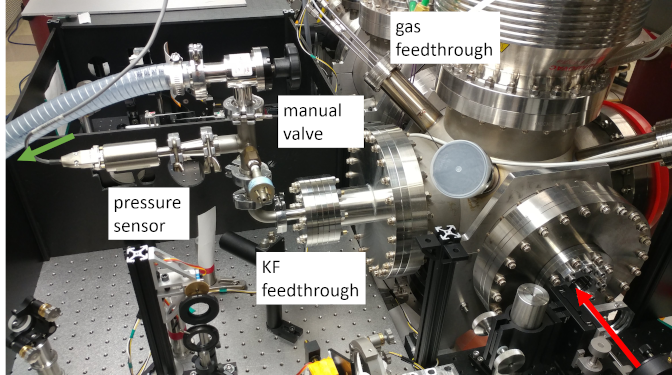
\includegraphics[width=0.9\textwidth]{figures/app1/HPC_outside_view_lowres.png}
	\caption{Exterior view of the generation chamber with the HPC installed showing the ancillary vacuum hardware. Red arrow indicates input laser path; green arrow points towards the HPC's RV pump.}
	\label{fig:HPC_outside_view}
\end{figure}

This section will discuss the initial setup and day-to-day operational details of the HPC. For the HHG \& pressure performance of the HPC, see \cref{sec:HPC}.

\Cref{fig:HPC_outside_view} is a picture of the exterior of the generation chamber, showing the ancillary vacuum hardware associated with the HPC. A small oil-lubricated RV pump (not shown) provides differential pumping to the interior of the HPC. An inline Baratron diaphragm pressure sensor (effective range: 1 -- 760 Torr) tracks the interior pressure of the edge-welded bellows. A manual gate valve is used to isolate the HPC from the RV pump when the additional pumping is not needed. Right angle KF fittings were used to route the HPC's vacuum line above the pump arm of the interferometer. The optics associated with the interferometer can be seen below this hardware on the optical table.

\subsection{Initial Installation and Alignment}
\label{app:initial-alignment-HPC}
First, a note about laser safety. As with all initial alignment procedures, the lowest possible laser power should be used to minimize both accidental laser drilling of the HPC components and the danger posed by stray light and back reflections. The surface most likely to cause laser scatter is the front face of the outer pipe, which is roughened stainless steel located about 3/8" before the focus. The material's roughness and the negative radius of curvature of the incoming light make it unlikely that incident light will coherently focus to a point upon reflection. However, it is possible that the sidewall of the outer pipe's aperture could act as a focusing mirror. Additionally, the hose clamp or mounting bracket could coherently reflect light towards the user. The user is advised to strictly follow all laser safety protocols during this alignment procedure. Whenever possible, direct observation of the laser beam on the surfaces of the HPC should be avoided, instead a remote sensor (webcam) should be used to view the interior of the generation chamber.

The initial installation of the HPC can be time consuming and tedious, but once installed it will retain its alignment indefinitely (weeks or months). As with a free expansion gas jet, fine adjustments to the pointing should be done on a daily basis. However, these adjustments will usually take less than 5 minutes.

Optically, the HPC cell consists of four pinhole apertures (diametrically opposed pinholes on both the inner and outer pipes) with the laser focus near the center of the inner pipe. The optical transmission of the HPC is therefore very sensitive to the relative alignment of these components, as well as the pointing of the laser into the HPC. To simplify the alignment, the two innermost holes are laser drilled \textit{in-situ} after the outer pipe's apertures have been aligned. To maintain the relative alignment of the inner \& outer apertures, the user should refrain from adjusting the inner pipe after the initial alignment is completed. Therefore, daily alignment of the HPC consists of moving all four apertures together via the in-vacuum motorized XYZ stages.

The first step of the HPC installation is installing the rough vacuum feedthrough flange. The TABLe's generation chamber uses a custom flange (a 4.5" CF blank with a KF16 half nipple welded to the air-side and a KF16 bulkhead groove \& tapped holes machined into the vacuum side). To accommodate the length of the in-vacuum bellows, we use a custom 10" CF to 4.5" CF reducing nipple (OAL = 4.25"), which acts as a spacer between the feedthrough flange and the KF16 flange on the HPC. Although it was absent from the original design, a spacer 4.5" CF flange (thickness = 0.68") between the feedthrough and the reducing full nipple is used to relax the compression in the bellows and allow for a larger range of motion. For convenience, the user should install the edge-welded bellows to the bulkhead flange before installing the flange on the chamber.

\begin{figure}
	\centering
	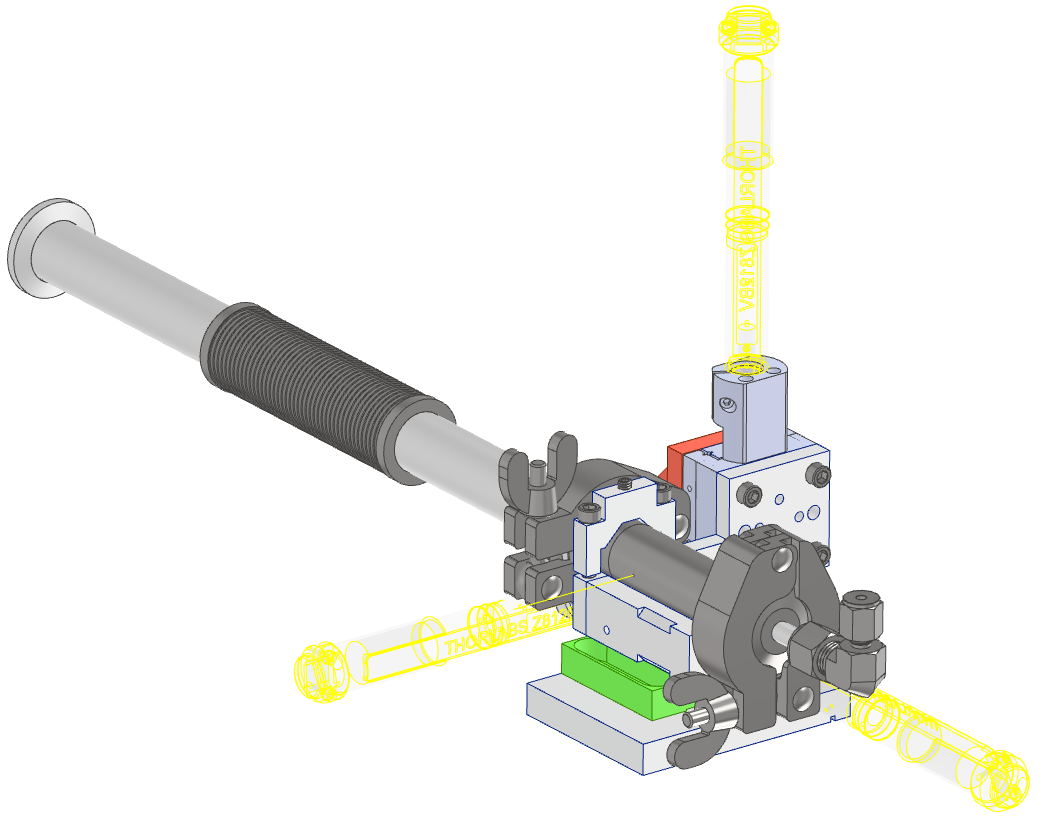
\includegraphics[width=0.9\textwidth]{figures/app1/HPC_on_stage2.png}
	\caption{The HPC with bracket installed on the XYZ translation stage, configured for the generation chamber. The hose clamp and gas supply tube are omitted from this drawing for clarity.}
	\label{fig:HPC_on_stage}
\end{figure}

The supporting bracket for the HPC was designed to be interchangeable with the free gas nozzle's bracket. See \cref{fig:HPC_on_stage} for details. This design allows the user to change the gas source type (HPC, LPC, or free expansion jet) without disturbing the alignment of the XYZ stage to the optical axis. For completeness, we will assume that the XYZ stage has been misaligned or removed from the chamber. First, the user should align the laser to the interferometer so that the laser path in the generation chamber can be used as a reference. Then, the stage should be positioned in the chamber so that the focus is roughly in the center of the stage's motion. Next, the stage's k-direction should made parallel to the optic axis. This can be done by tracking the position of the laser on a card mounted to the stage while moving the stage upstream and downstream of the focus. After clamping the stage to the breadboard, check that the alignment is still true before continuing to the next step.

Now that the XYZ stage is aligned to the laser, we will install the outer pipe of the HPC and align its apertures to the laser. We do so by maximizing the light transmission through the apertures. This is best done in two steps: first, coarse alignment is done visually at low power (insufficiently intense to laser drill the pipe), followed by fine adjustments using a power meter at moderate intensities (above the noise floor of the power meter). Note that drilling out the outer pipe's apertures will lessen the alignment requirements at the expense of the HPC's differential pumping performance. Given the chamber's small internal dimensions, it is not practical to place a power meter in the generation chamber after the focus during the alignment procedure. Rather, it is preferable to divert the beam out of the vacuum system using the linear actuator \& silver mirror assembly located approximately 85 cm downstream of the focus.\footnote{Special thanks to Eric Moore for designing and installing this optomechanical component.} When inserted, the linear actuator intersects the beam path and redirects the beam out of the vacuum system through a window onto the upper deck of the optical table. Note that for most generation focusing conditions, the large beam size at the diverting mirror makes this beam path lossy. To accurately calculate the transmission through the HPC, it is necessary to measure the power immediately after the HPC in the generation chamber.

For the coarse alignment, the input beam intensity should be reduced using an upstream iris, to the point that it is barely visible near the focus. Since a tightened KF connection prevents rotation of the components, the alignment of the outer pipe is done prior to making any KF connections. However, the KF clamps should be fitted on either end of the pipe to ensure that there is enough room to make the connections without disturbing the alignment once finished. The outer pipe should be placed in its cradle, with the aluminum \& hose clamps made snug around the pipe but not taut.\footnote{The HPC's XYZ assembly and bracket were designed for the TABLe generation chamber. If it is being installed elsewhere, the user should verify that the height is correct. When installed correctly, the bottom of the Z-motor range should correspond to the HPC lowered completely out of the way of the laser; the top of the range should correspond to the laser going through the center of the HPC, with about 1 mm to spare.} Transmission should be optimized by iteratively tuning the following parameters: (1) rotation of the pipe in the cradle, (2) height of the cradle using the vertical motor, and (3) horizontal (transverse) position of the assembly using both the horizontal motor and the position of the pipe in the cradle. For fine adjustment, the iris should be adjusted so that the power meter reads about 20--30 mW when measured after the linear actuator.\footnote{This power is appropriate for a 1 kHz repetition rate and a generation focal length of 30 or 40 cm.} The clamps should be tightened so that movement of the pipe is possible, but difficult. The area around the power meter should be covered to prevent air currents from affecting the measurement. The transmitted power should be optimized using the same procedure as before.

\begin{figure}
	\centering
	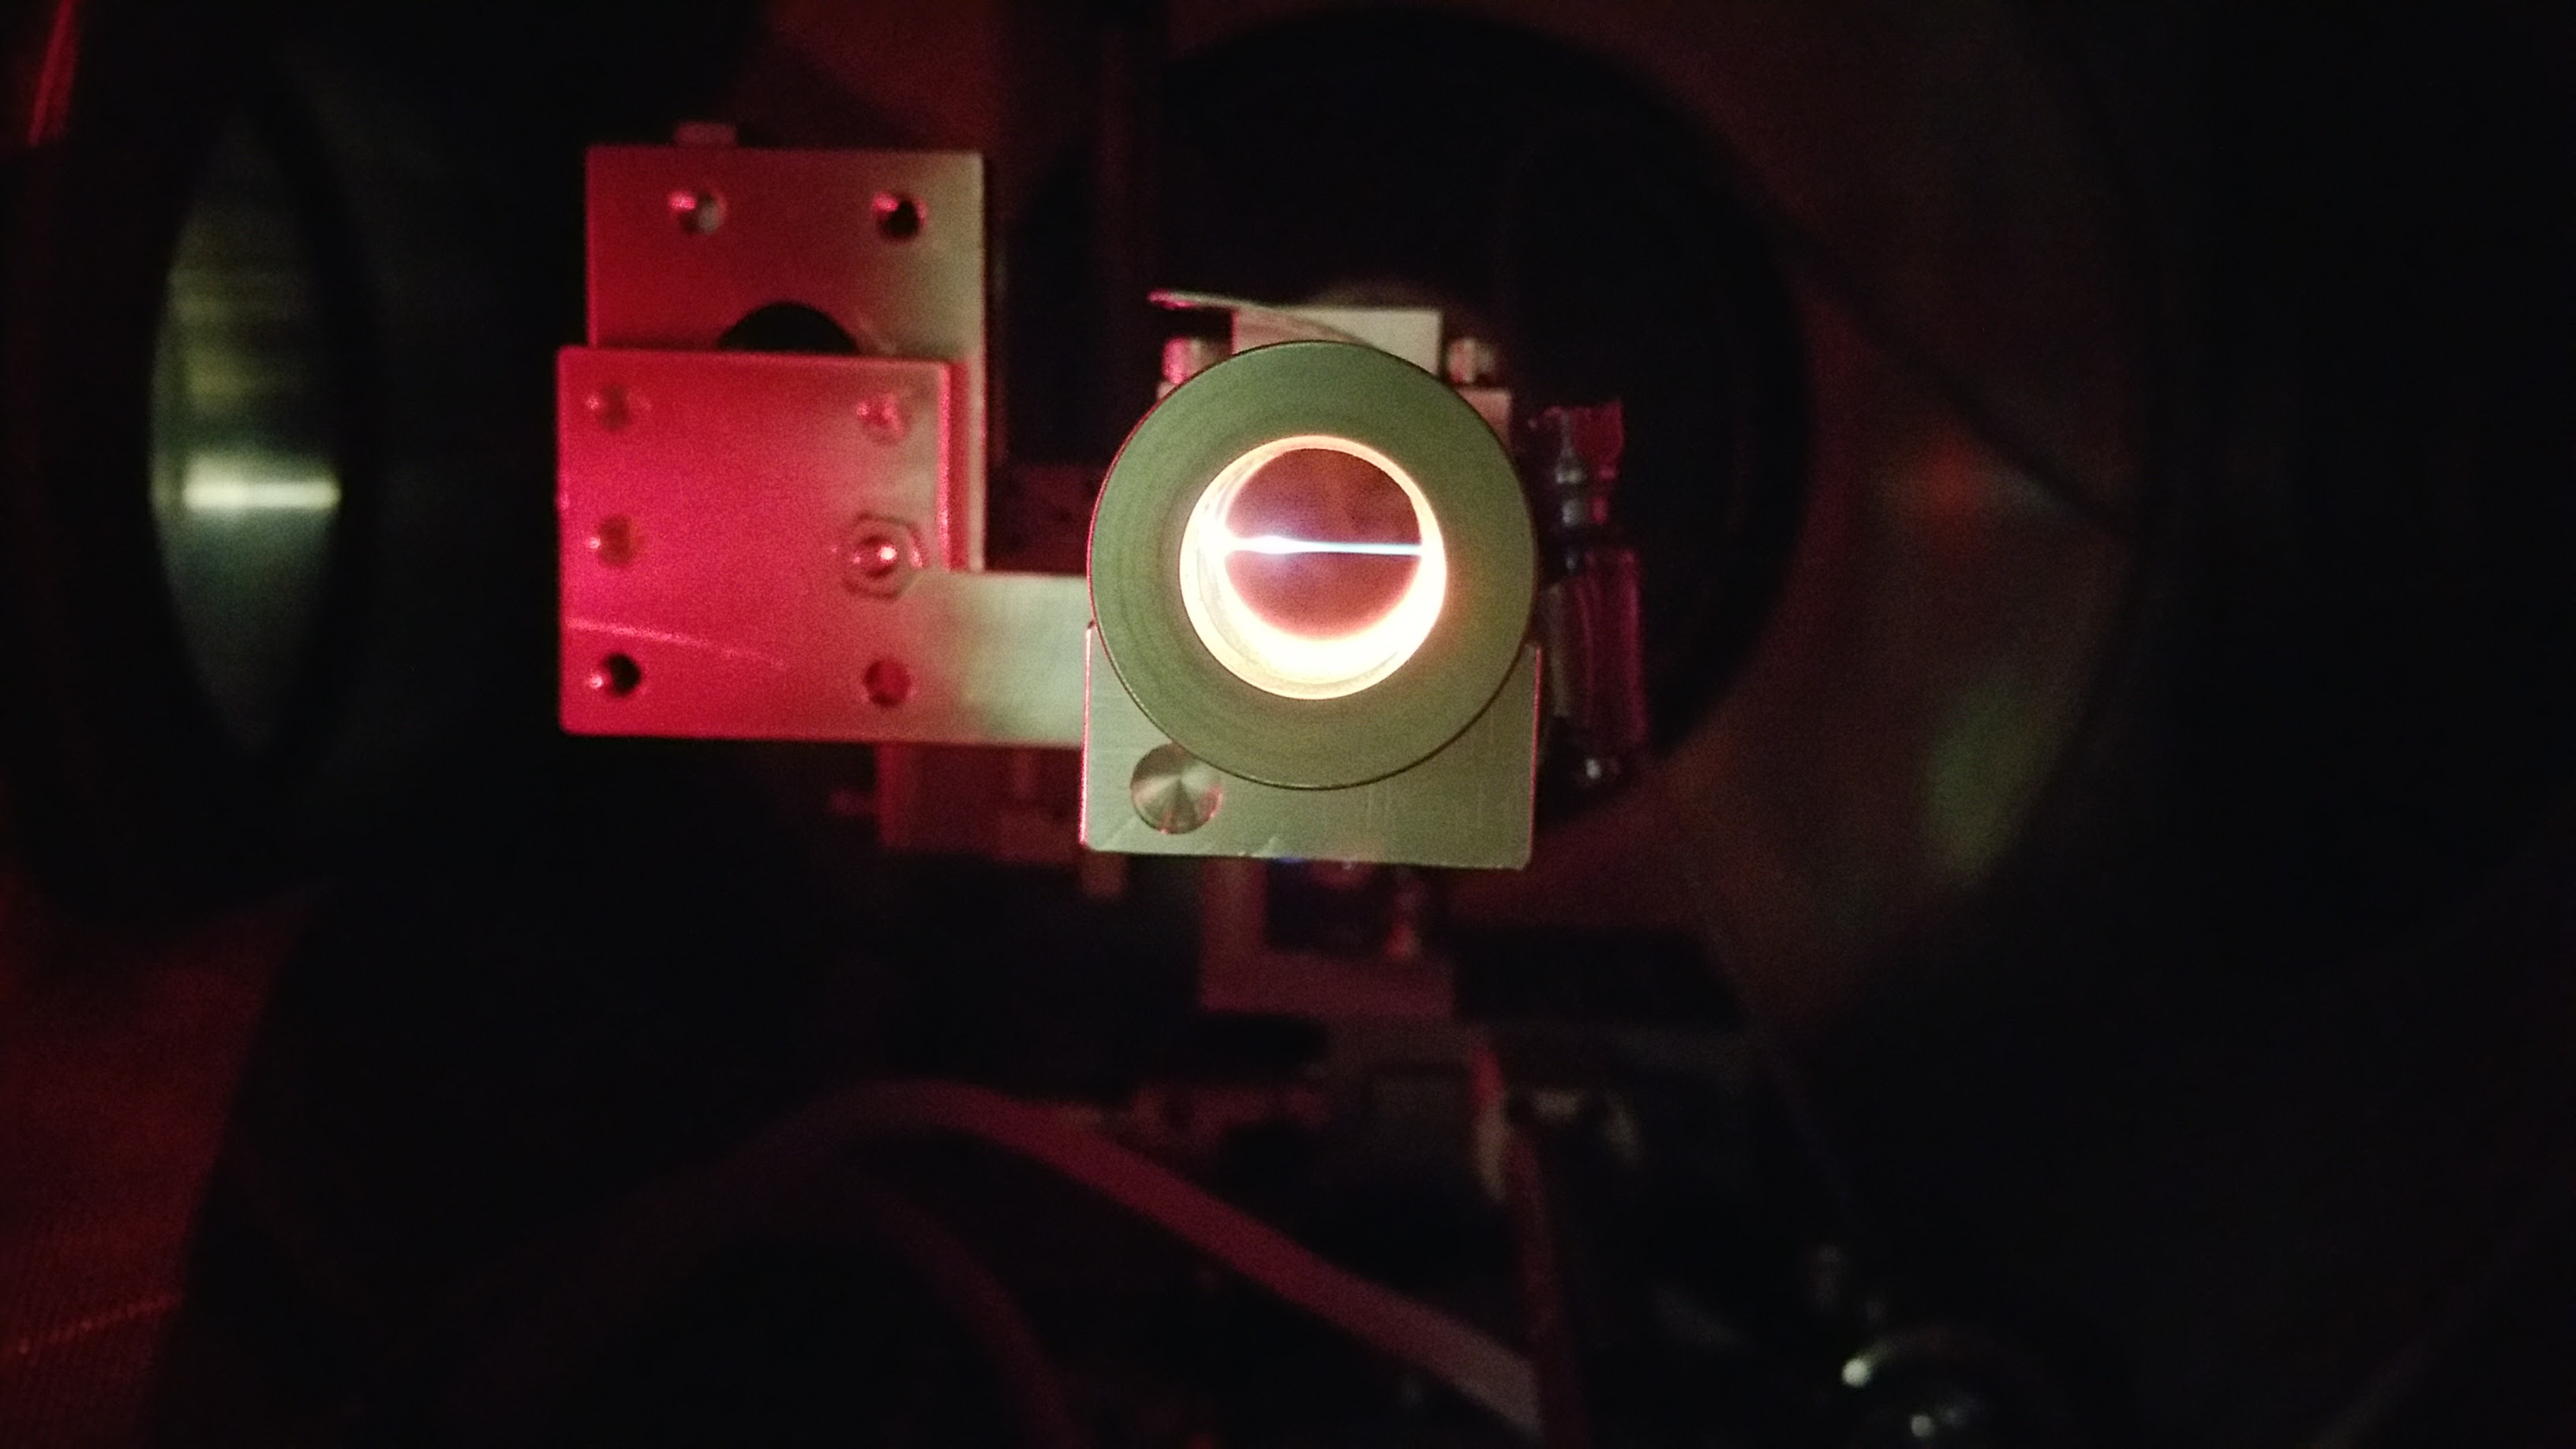
\includegraphics[width=0.9\textwidth]{figures/app1/HPC_outer_can_laser.jpg}
	\caption{Laser filament in the aligned outer pipe of the HPC. The inner pipe is not yet installed. Alignment of the outer pipe is done at very low intensities; after alignment the power was increased to create a filament for illustrative purposes only. This picture was taken in the target chamber during the initial testing of the HPC. The geometry of this chamber requires that the orientation of the mounting bracket is reversed compared to what is shown in \cref{fig:HPC_on_stage}.}
	\label{fig:HPC_outer_can_laser}
\end{figure}

Once the outer pipe is aligned, tighten all connections and connect the bellows to the outer pipe. Check that the alignment has not been changed by torquing these connections. Verify that the unattenuated laser beam can pass through the outer pipe without interference, as shown in \cref{fig:HPC_outer_can_laser}. 

Next we install the inner pipe. First, attach the gas delivery feedthrough flange onto the HPC assembly without the inner pipe. Being mindful to not disturb the alignment of the outer pipe, check that the gas delivery tubing does not interfere with the laser path. Remove the gas delivery feedthrough flange, cut the inner pipe to length (OAL = 1.75"), and make the Swagelok connection between the inner pipe and the KF feedthrough. Make sure the inner pipe is normal to the flange's sealing surface, otherwise the laser will skim the sidewall of the inner pipe rather than go through the center. If this happens, the laser-gas interaction length will be reduced and the HHG performance of the system will suffer. Install the gas delivery assembly onto the HPC assembly by tightening the KF clamp.

Laser drilling the inner pipe will sputter a significant amount of metal onto the inner surfaces of the chamber. It is therefore important to protect the optics from the resulting metal plume. Since the active drilling surface is on the upstream face of the pipe, most of the material will go upstream. Therefore, the laser window needs to be swapped out for a "sacrificial" window prior to drilling.\footnote{Using a window with different optical properties (i.e., thickness or material), or no window at all, will change the pointing and effective focal length of the beam. It has been suggested that the laser window could be protected by placing a thin sheet of transparent plastic between the window and the HPC, but this method has not been tested.} Out of an abundance of caution, close the gate valve to the mirror chamber, retract the linear actuator \& silver mirror from the beam path, and block the generation chamber's vacuum aperture with a card.

Laser drilling should be done with the appropriate safety precautions: wearing laser goggles, notifying coworkers of your activity, and posting signs on the entrances to the lab to reduce unnecessary foot traffic. The user can cover up the chamber's flanges and set up a webcam to remotely monitor the laser drilling status to minimize the risk of inadvertent laser exposure.

\begin{figure}
	\centering
	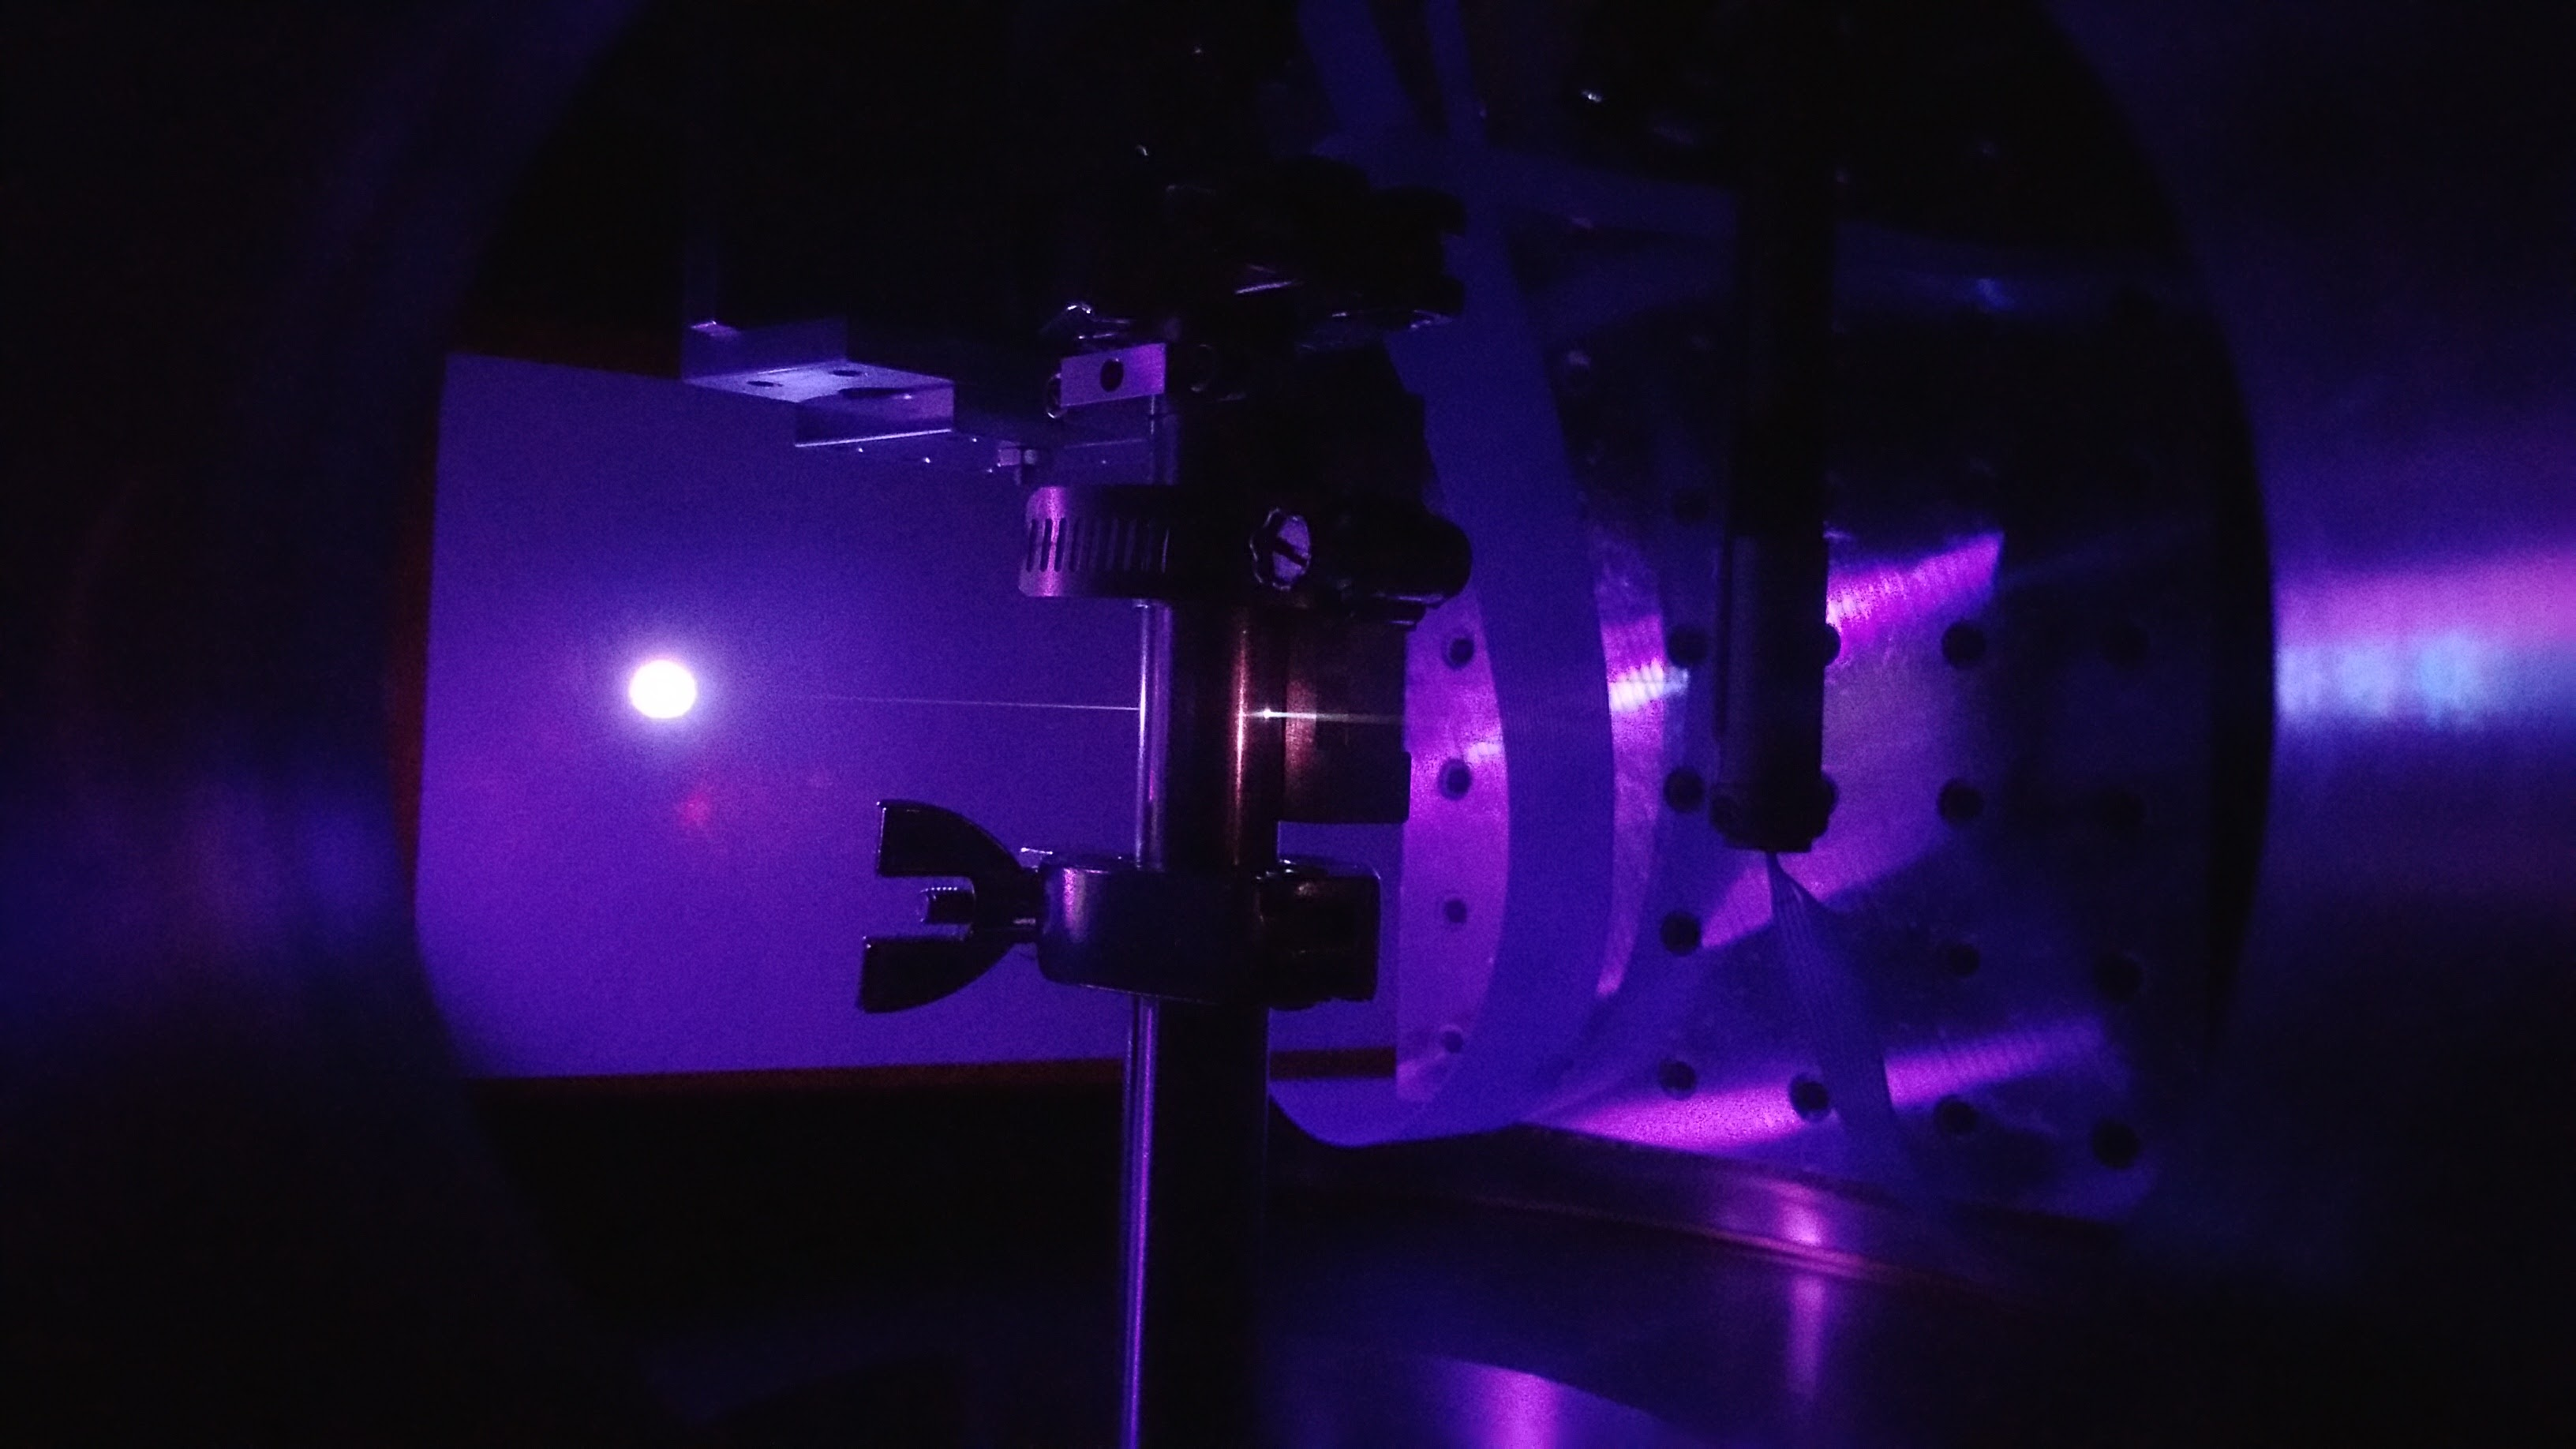
\includegraphics[angle=270, width=0.75\textwidth]{figures/app1/HPC_drilling.jpg}
	\caption{Laser drilling the inner pipe. A card blocks the laser after exiting the HPC. The HPC was pressurized with Ar gas to enhance the filament for illustrative purposes.}
	\label{fig:HPC_drilling}
\end{figure}

At this point, the actual process of laser drilling is quite simple. There is no way to control the exact positioning of the inner pipe relative to the outer pipe, so there are no adjustments to make. Rather, the design relies on the mechanical alignment of the inner pipe relative to the outer pipe, which is ultimately set by the gas feedthrough weld, the Swagelok / KF fittings. On the other hand, a used inner pipe cannot be reinstalled to the HPC once it is removed, since alignment is effectively impossible. To laser drill the pipe, simply let the unattenuated beam into the chamber and wait a few minutes until the laser emerges from the exit of the HPC. See \cref{fig:HPC_drilling}.

If you are planning on scanning the k-direction of the HPC during an experiment, you should do so now while you are set up for laser drilling. Similarly, if you are using a chromatic focusing scheme and are planning on changing wavelengths during your experiment (which will change the effective focal length), you should step through the full range of wavelengths while drilling. Doing so will open up the apertures slightly, resulting in additional metal deposition on the sacrificial laser window and reduced HPC pressure performance.

After laser drilling is complete, reinstall the laser window and verify the HPC has retained its alignment.

\subsection{Alignment with the HPC Installed}

Once lowered out of the beam path, the HPC does not affect the daily pointing procedure. However, there are some extra considerations that need to be made if the HPC is installed. The small apertures of the HPC and the non-linear nature of HHG demand high accuracy in the pointing into the cell, so small corrections to the positioning of the HPC have to be made after the daily pointing procedure is completed.

\subsubsection{Pointing into the Interferometer}
If the interferometer is already aligned, the presence of the HPC does not really complicate the daily procedure of the beamline. In this case, the user should block the laser into the generation chamber and align the pointing into the interferometer using the pump arm, via the standard procedure.\footnote{Failure to block the laser prior to changing the pointing may result in laser-drilling the HPC.} Since harmonic generation is extremely sensitive to pointing, the user may have to make small tweaks to the transverse position of the HPC after a nominal alignment of the interferometer. This can be achieved by setting a fast camera exposure ($< 0.5$ s) and optimizing HHG yield with respect to the HPC vertical \& horizontal position (take 10 - 25 $\mu$m steps). In our experience, the optimal HPC position is typically within {50 $\mu$m} of the previous day's position.

The HPC's apertures may no longer be circular if the HPC has been subjected to accidental laser drilling or significant laser drift. Non-circular apertures may result in a complex spatial profile of the harmonics, which can make the optimization of the harmonic yield difficult.

\subsubsection{Aligning the Interferometer}
If the interferometer needs to be realigned, then the HPC must be lowered out of the way of the laser path. Unless major changes were made to the interferometer, the angle of the HPC's apertures should remain aligned to the k-vector of the generation arm. In this case, the optimal position of the HPC can be found by maximizing the transmitted power of an the attenuated laser through the HPC, as described in the latter part of \cref{app:initial-alignment-HPC}. If major modifications were made to the interferometer, the user should consider aligning the HPC from scratch.


\subsection{Using the HPC}

The extra vacuum pump adds complications to the TABLe operating procedures described in \cref{sec:OMRON_instructions,sec:OMRON_venting}. Before pumping the TABLe down from atmosphere, ensure the HPC's manual value (see \cref{fig:HPC_outside_view}) is closed.

Increase the backing pressure until the internal bellows pressure reaches $\sim$20 Torr, or until the generation chamber reaches $\sim$3 mTorr (whichever happens first). Then, turn on the HPC's RV pump and slowly open the external manual valve. The pressure inside the system should drop. This order of operations ensures the net gas flow direction will be into the RV pump rather than the generation chamber, minimizing the chance of oil contamination in the main TABLe apparatus. Once the HPC's vacuum pump is running, the user can continue increasing the backing pressure until the operating pressure is reached. \textbf{Note that the pressure differential between the inside of the HPC's bellows and the generation chamber cannot exceed 120 Torr without risking damage to the HPC's bellows.} The shutdown procedure follows the same steps, but in reverse. Lower the backing pressure to the HPC until the generation chamber pressure is $\sim 5 \times 10^{-4}$ Torr, then close the manual valve to the HPC's RV pump. Once the valve is closed, shut off the gas completely and turn off the RV pump. The TABLe system is now ready to be vented (\cref{sec:OMRON_venting}), or left idle.

%For daily alignment, insert the diagnostic mirror into the beam path and measure the transmitted power of an attenuated beam. If the recorded number is lower than expected, optimization can be performed by using the HPC's vertical \& horizontal motors. Once satisfied with the initial alignment, we can begin to let the generating gas into the chamber. Starting with zero backing pressure, open the gas valve to the inner pipe. This will cause the pressure of the inner pipe and the generation chamber to quickly rise, then stabilize. 

%\subsection{Startup and Shutdown}


%\section{Laser System Specifics}
%importance of pointing \& laser performance for our experiments
%
%\subsection{The Spitfire}
%\subsubsection{Regular Maintenance}
%- cleaning the stretcher
%
%- increasing the pump laser currents
%
%- changing the chiller fluid, desiccants, etc
%
%\subsubsection{quirks and features}
%- regen cavity tweaks
%
%- photodiode problems
%
%- software issues - bugs and troubleshooting
%
%\subsection{Pointing Stabilization into the External Compressor}
%- dietrich plots for pointing
%\subsection{The Spitfire's External Compressor}
%\subsubsection{external compressor alignment}
%\subsubsection{cleaning the grating}
%
%\subsection{The TOPAS-HE}
%- aligning
%- importance of power stability and pointing stability
%
%\subsection{stability}
%- boxing things up
%- power stability throughout the day, people in the lab
%- unstable harmonic yield from the HPC at high pressures
%\section{The Shutter System}
%
%\section{The Vacuum System}
%- blower upgrade
%
%- remote pressure sensing
%
%- vacuum calculations for steady state pressure of beamline
%
%\section{Required Maintenance}
%
%vacuum system (rough pumps, blowers, turbos) and spitfire (cleaning the gratings)
%
%\section{Best practices: data acquisition}
%
%read-out noise from camera. (how noise scales)

